\chapter{Result and Discussion} % Main chapter title

\label{Chapter2.75} % Change X to a consecutive number; for referencing this chapter else where, use \ref{ChapterX}
%----------------------------------------------------------------------------------------
%	SECTION 1
%----------------------------------------------------------------------------------------

%-----------------------------------
%	SECTION 2
%-----------------------------------
\section{Before surface treatment}

Normalized cross-correlation evaluates the similarity between 2 patterns, the closer to 1, the higher the similarity. Here we compare the time-resolved PL spectra from every time tick with the first spectrum, the average value of this series of normalized cross-correlation reflects the general level of spectral stability of the measured point, additionally,the standard deviation of normalized cross-correlation indicates the speed of spectral changes.


\begin{figure}[h]
	\centering
	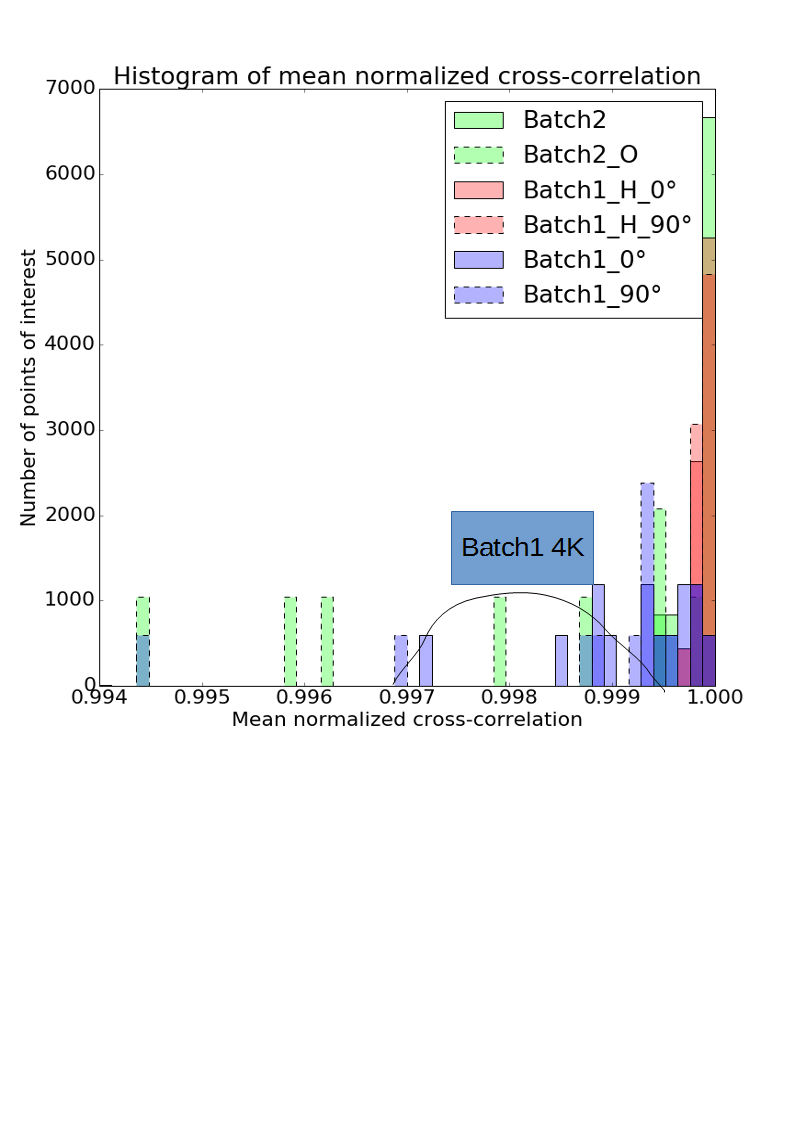
\includegraphics[width=1\linewidth]{Figures/pic/histall}
	\caption{Normalized histogram of mean normalized cross-correlation.}
	\label{fig:2015-09-07-ow-capture-20150907151210-744-1}
\end{figure}

Normalized cross-correlation evaluates the similarity between 2 patterns, the closer to 1, the higher the similarity. Here we compare the time-resolved PL spectra from every time tick with the first spectrum, the average value of this series of normalized cross-correlation reflects the general level of spectral stability of the measured point, additionally,the standard deviation of normalized cross-correlation indicates the speed of spectral changes.

As can be seen in Fig. 5.1, batch2 has better spectral stability than batch1. Larger diamond has better spectral stability fits the prediction that the spectral diffusion is related to the surface band bending. 

\paragraph{power dependency}
\begin{figure}[h]
\centering
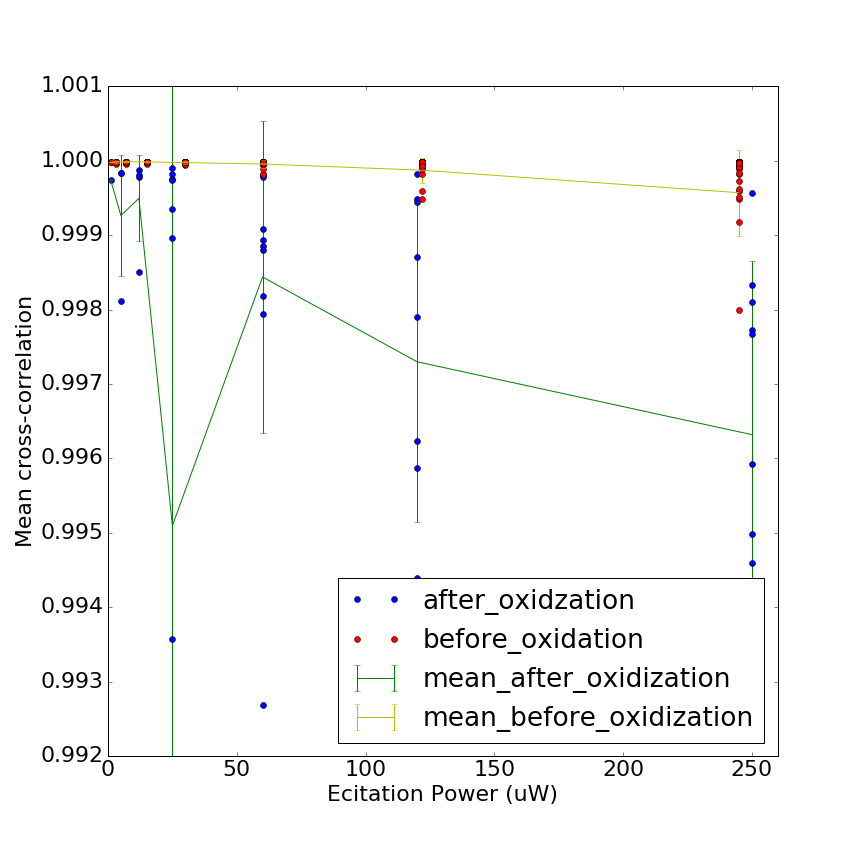
\includegraphics[width=0.7\linewidth]{Figures/pic/powerdependencybeforeafteroxidation}
\caption{Powerdependency of nanodiamond batch2, before and after first oxidation.}
\label{fig:powerdependencybeforeafteroxidation}
\end{figure}

\paragraph{temprature dependence}



\paragraph{excitation polarisation}


\begin{figure}[h]
\centering
\includegraphics[width=0.7\linewidth]{"Figures/pic/excitation polarisation"}
\caption{Mean normalized cross-correlation against excitation polarisation. The error bar stand for standard deviation}
\label{fig:excitation-polarisation of untreated nanodiamond batch 2}
\end{figure}

\section{Hydrogen termination}


